
\documentclass{beamer}
\mode<presentation>
\usepackage{amsmath}
\usepackage{amssymb}
%\usepackage{advdate}
\usepackage{graphicx}
\graphicspath{{../Figs/}}
\usepackage{adjustbox}
\usepackage{subcaption}
\usepackage{enumitem}
\usepackage{multicol}
\usepackage{mathtools}
\usepackage{listings}
\usepackage{url}
\def\UrlBreaks{\do\/\do-}
\usetheme{Boadilla}
\usecolortheme{lily}
\setbeamertemplate{footline}
{
  \leavevmode%
  \hbox{%
  \begin{beamercolorbox}[wd=\paperwidth,ht=2.25ex,dp=1ex,right]{author in head/foot}%
    \insertframenumber{} / \inserttotalframenumber\hspace*{2ex} 
  \end{beamercolorbox}}%
  \vskip0pt%
}
\setbeamertemplate{navigation symbols}{}
\let\solution\relax
\usepackage{gvv}
\lstset{
%language=C,
frame=single, 
breaklines=true,
columns=fullflexible
}



\begin{document}



\title{6.4.2}
\author{AI25BTECH11002 - Ayush Sunil Labhade}
{\let\newpage\relax\maketitle}


\textbf{Question}: Find the shortest distance between the lines:\\
\begin{center}
	$\vec{r} = 4\hat{\imath} - \hat{\jmath} + \lambda(1\hat{\imath} + 2\hat{\jmath} -3\hat{k})$\\
$\vec{r} = \hat{\imath} - \hat{\jmath} + 2\hat{k}+ \mu(2\hat{\imath} + 4\hat{\jmath} -5\hat{k})$
\end{center}



\textbf{Solution:}\\
Let $\vec{x}_1$ and $\vec{x}_2$ be the points on the given lines respectively.\\
$\vec{x}_1 = \myvec{4 \\ -1 \\ 0} + \lambda\myvec{1 \\ 2 \\ -3}$ and $\vec{x}_2 = \myvec{1 \\ -1 \\ 2} + \mu\myvec{2 \\ 4 \\ -5}$\\
Let $\vec{A} = \myvec{4 \\ -1 \\ 0}$ and $\vec{B} = \myvec{1 \\ -1 \\ 2}$\\
Let $\vec{M} = \myvec{1 & 2 \\ 2 & 4 \\ -3 & -5}$\\

\begin{align}
(\vec{M} \, \, \vec{B}-\vec{A}) = \myvec{1 & 2 & -3 \\ 2 & 4 & -1 \\ -3 & -5 & 2}
\end{align}

Row Transformation-1: $R_2 \rightarrow R_2 - 2R_1$
\begin{align}
\myvec{1 & 2 & -3 \\ 0 & 0 & 5 \\ -3 & -5 & 2}
\end{align}

Row Transformation-2: $R_3 \rightarrow R_3 + 3R_1$
\begin{align}
\myvec{1 & 2 & -3 \\ 0 & 0 & 5 \\ 0 & 1 & -7}
\end{align}

Row Transformation-3: $R_3 \leftrightarrow R_2$
\begin{align}
\myvec{1 & 2 & -3 \\ 0 & 1 & -7 \\ 0 & 0 & 5}
\end{align}

Therefore, The Rank is 3 $\Rightarrow$ The Lines are Skew Lines.\\

\begin{align}
\text{Let } \vec{K} = \myvec{\lambda \\ -\mu}
\end{align}

\begin{align}
(\vec{M}^\top\vec{M})\vec{K}=\vec{M}^\top(\vec{B-A})
\end{align}

\begin{align}
\myvec{14 & 25 \\ 25 & 45}\vec{K} = \myvec{-9 \\ -15}
\end{align}

The Augmented Matrix from Equation 6,\\

\begin{align}
\augvec{2}{1}{
14 & 25 & -9\\
25 & 45 & -15
}
\end{align}

After Row Reductions,
\begin{align}
\augvec{2}{1}{
1 & 0 & 3\\
0 & 1 & -\dfrac{9}{5}
}
\end{align}

\begin{align}
\therefore \, \vec{K} = \myvec{3 \\ -\dfrac{9}{5}}
\end{align}

\begin{align}
\therefore \, \lambda = 3 \, \text{and} \, \mu = \dfrac{9}{5}
\end{align}

From Equation 10,
\begin{align}
\vec{x}_1 &= \myvec{4 \\ -1 \\ 0} + 3\myvec{1 \\ 2 \\ -3} = \myvec{7 \\ 5 \\ -9} \\
\vec{x}_2 &= \myvec{1 \\ -1 \\ 2} + \dfrac{9}{5}\myvec{2 \\ 4 \\ -5} = \myvec{\dfrac{23}{5} \\ \dfrac{31}{5} \\ -\dfrac{23}{5}}
\end{align}

The Minimum Distance between the given skew lines is $\norm{\vec{x}_2 - \vec{x}_1}$\\
\begin{align}
\norm{\vec{x}_2 - \vec{x}_1} = \sqrt{(\vec{x}_2 - \vec{x}_1)^\top (\vec{x}_2 - \vec{x}_1)} = \dfrac{13}{\sqrt{5}}
\end{align}

The Minimum Distance between the given Lines = $$\dfrac{13}{\sqrt{5}} $$
\newline

Graph:
\begin{figure}[H]
    \centering
    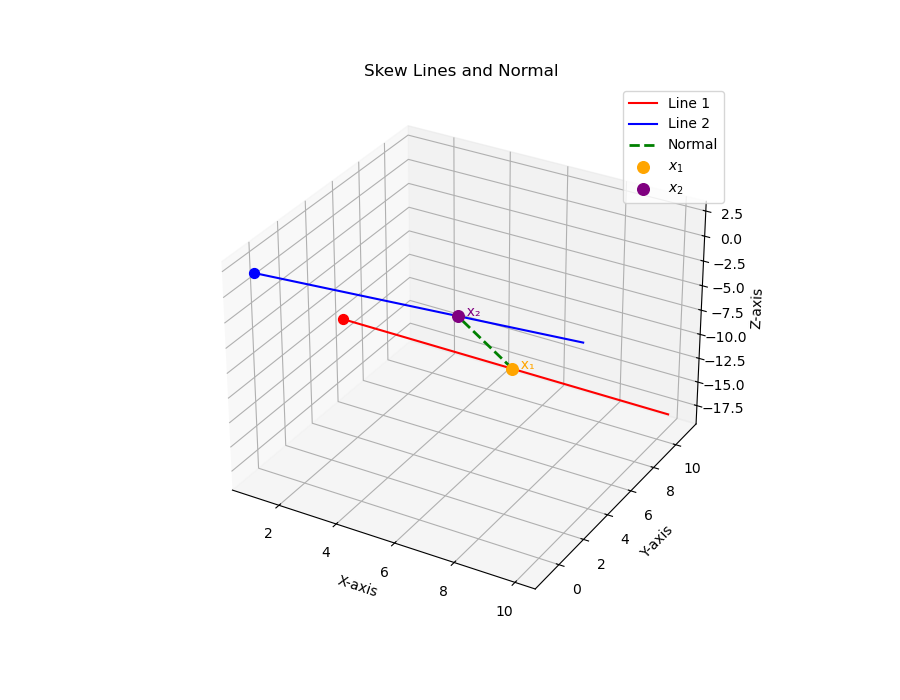
\includegraphics[scale=0.5]{plot}
    \caption{}
    \label{fig:plot}
\end{figure}
\end{document}
